\documentclass{bioinfo}

\usepackage{float}
\usepackage{natbib}
\usepackage{url}
\usepackage{har2nat}
\usepackage{listings}

\copyrightyear{2017} \pubyear{2017}

\access{Advance Access Publication Date: 24 March 2017}
\appnotes{Protein Prediction}

%\bibliographystyle{natbib}
%\bibliographystyle{achemnat}
%\bibliographystyle{plainnat}
%\bibliographystyle{abbrv}
%\bibliographystyle{bioinformatics}
\bibliographystyle{plain}

\begin{document}
\firstpage{1}
\subtitle{Bioinformatics - Prof. David T. Jones}
\title[Predicting Localization]{Predicting Subcellular Localization of Eukaryotic Proteins}
\author[Clarke]{Andrew Clarke\,$^{\text{\sfb 1,}*}$}
\address{ $^{\text{\sf 1}}$CS, University College London, London, WC1E 6BT, UK.}
\corresp{$^\ast$To whom correspondence should be addressed.}
\history{Accepted on March 24, 2017}
\editor{Associate Editor: Andrew Clarke}

\abstract{\textbf{Motivation:}
Sequencing genomes without understanding the role of those genes is of little value.
We need to understand how the components of a genome affect health, growth, and life in general.
The first step to understanding a specific genes role in our lives is understanding the role of its corresponding protein.
Accurately predicting the subcellular location of a given protein, based on its DNA sequence, is a key element.
This paper investigates and implements some techniques for predicting the subcellular location of proteins given their amino acid sequence.\\
\textbf{Results:} Using amino acid statistics, dipeptide statistics, and chemical properties, I was able to predict the subcellular location of eukaryotic proteins in an effective manner.\\
\textbf{Availability: Yes} \\
\textbf{Contact:} \href{andreweskeclarke@gmail.com}{andreweskeclarke@gmail.com}\\
\textbf{Supplementary information:} Supplementary data are available on request.}

\maketitle

\section{Introduction}

As sequencing genomic data becomes cheaper and more common, there is a growing need to effectively infer the function of those genes.
Predicting function aides diagnosing dysfunction from genetic mutations, and in developing therapies.
Having an efficient computational model to predict the function of genes from sequencing data would be ideal.
A computational model could ensure function assignment scales at the same rate as gene discovery.

Being able to infer the function of a gene means inferring the function of its corresponding protein.
One key aspect of understanding a protein's role in an organism is to understand where it is used, its subcellular localization.
This is the topic this paper focuses on.

There is a long history of predicting subcellular location using computaitonal models.
Many successful models are shared online, like at \url{http://www.psort.org} and \citep{meinken_subcellular_2017}.
The long history and range of solutions comes about from the large number of choices when predicting protein location.
The choices include the types of organisms, the number of location classes, the features used, the type of model, etc.

For example, Gao (2005) \cite{gao_prediction_2005}, whose approach I am following most closely, uses n-nearest neighbors with a custom distance metric.
Nearest Neighbors creates a very non-linear boundary between proteins in a high dimensional feature space.
When predicting a proteins location, the model finds the n most similar proteins it has seen before.
These similar proteins, whose locations are known, ``vote" on the location of the new protein.
The custom distance metric allows emphasizing certain features over others.

Recurrent Neural Networks (RNNs), and especially the Bidirectional LSTM models, have also found success in subcellular location prediction \citep{thireou_bidirectional_2007}.
RNNs learn features directly from sequences, removing the need for manual feature engineering.
Basic LSTM models run through a sequence in one direction, while the bi-directional model is more applicable to the bidirectional dependencies in protein sequences.

Even with the success of neural networks, there are still benefits from intelligent feature selection.
Thinking more deeply about the movement of proteins within organisms leads to signal peptide matching \citep{nielsen_identification_1997}.
Specific peptide sequences are used by the cell to identify mitochondrial proteins, secretory proteins, chloroplast proteins, etc.

Thinking more deeply about the evolution of different proteins leads to a phylogenetic approach.
If two proteins have an inferred evolutionary relationship, it is likely they have similar functions and work in similar locations.
Indeed, Marcotte et al. 2000 \cite{marcotte_localizing_2000} found success in predicting mitochondrial proteins based on phylogenetic features.

In this paper I will use features derived from previous knowledge about proteins.
I compare the accuracy of several machine learning models under different feature sets.

\section{Approach}

For this paper, I am limiting the focus narrowly.
The data and predictions are for eukaryotic cells only.
There are only four locations to predict, (1) Cytosolic, (2) Secreted, (3) Nuclear, (4) Mitochondrial

I am only using three sets of features: single amino acid statistics, dipeptide statistics, and physicochemical properties.
The amino acid statistics consist of raw amino acid counts in a sequence.
The dipeptide statistics are raw counts of amino acid pairs in a sequence.
Interestingly, I found counts to be more informational than averages in both cases.
The physicochemical properties were taken from AAindex \citep{genomenet_aaindex_2017}, and the properties I chose were inspired from \citep{gao_prediction_2005}, which in turn have been used since the 1970s.
The nine properties are:
\begin{enumerate}[(1)]
  \item
    Flexibility - a measure of the flexibility an amino acid allows in the secondary structure. A rigid amino acid would cause straight chains in the secondary structure. For example glycine's structure allows the secondary structure to hinge widely, while restrictive, less flexible amino acids like proline limit the possible structures at that point.
  \item
    Refractivity - an optical property of amino acids.
  \item
    Volume - the size of the amino acid, and especially important to know the total sum in a sequence. This is one of the more useful properties
  \item
    Free energy -the free energy of the amino acid.
  \item
    Electron ion interaction - the susceptibility of certain types of molecular bonds between amino acids.
  \item
    Hydrophilicity - how favorable a protein is to water, indicating, for example, whether it is likely to be found in the cytoplasm or not.
  \item
    Polarity - how polar an amino acid is, affects its affinity for polar bonds.
  \item
    Hydrophobicity - how unfavorable a protein is to water, indicating the opposite of the hydrophilicity.
  \item
    Isoelectric point - measures the pH of a system, and is important in its sum total.
\end{enumerate}

\section{Methods}

In this section I will discuss details of the feature manipulations and model training.

\subsection{Features}

I created a set of garbage features, just random numbers, to test the lower limits of accuracy for each model.
Each should be around 25-35\%. 25\% would correspond to random guessing, and 35\% corresponds to guessing 'nucleus' every time.
Since nucleus is the most common location in our data, this is an artifact of data collecton.

The most simple real features I started with were merely sequence length and protein mass.

The next set of features were physicochemical features.
They were combined in three different ways.
First, the sequence of amino acids was converted into a sequence of the properties, e.g. a list of amino acid volumes.
Then, the sum of that list, the mean of that list, and the auto correlation of that list was incorporated into our training data.
The sum and mean were included as they are the most simple summaries for the overall protein. 
Auto correlation was included due to its reported predictive power.

One important note is that these sequences vary in length.
The length information is partially encoded in the sum of properties.
The longer chains will have higher sums.
Using only the mean would drop most length information.

The auto correlation was inspired by \cite{gao_prediction_2005}.
The auto correlation $r_k$ for a single sequence of length n is given by, looking back k steps:
\[  \frac{\sum_{i=k}^n(p_i - \bar{p})(p_{i-k} - \bar{p})}{ \sum_{i=k}^n(p_i - \bar{p}) } \]
I took the autocorrelation looking back between 1 and 5 steps for each physicochemical property.
There was no specific intuition behind this choice, except that I wanted to avoid an overly large number of features.
Once our feature set grows too large, say on the order of how much data we have, overfitting becomes a huge problem.

The third set of features were single amino acid counts.
For the 20 amino acids, plus three additional codes in the data, I incorporated the raw count within a sequence as a feature.
This amounts to 23 additional features.

The fourth set of features were amino acid pair counts (dipeptide counts).
This amounted to 529 additional features.

\subsection{Models}

I tried a number of models to gauge which might work well.

When doing classification, the first question we always ask is "does logistic regresson work?"
Logistic regression looks for the best linear relationship between all the features, and computes a probability for each possible class.
If the relationship between the features is roughly linear, then the model will work well.
Otherwise, we need to be clever about manipulating our features.
We may need to add interaction terms between features.
Some features might have bad scaling, they may be on a log scale or an exponential scale for example.

The two other models I played with are non parametric, they do not assume a functional form between the features and the classes.

The first model is gradient boosted trees.
Gradient boosted trees are similar to random forests, but each new tree does not train on the original data.
Each decision tree $T_m$ in the sequence fits the errors (residuals) from the previous $\{T_1,\dots,T_{m-1}\}$ trees.
At each step $T_m$ is added to the ensemble of the previous trees.
I chose the max depth of each tree to be 4, which allows the model to incorporate interactions between several features per tree.

Like \cite{gao_prediction_2005}, I also tried a simple K-Nearest Neighbor appraoch.
This looks for past proteins that are very similar to the protein we want to predict, and has them vote on the correct class.
I used the canberra distance metric to decide what "very similar" means.
It gives a rough similarity measure between each feature independently, similar to the cosine distance.
Since the scales of each feature are different, a simple Euclidean distance metric is inappropriate.

\subsection{Training}

Each model was trained using 10-fold cross validation.
The data was shuffled randomly, and then split into 10 folds.
The model was trained on 9 folds, and tested on the remaining validation fold.
This process was repeated 10 times, and the average accuracy over all validations was recorded.

\begin{table}
\caption{Cross Validated results by model and feature set}
\label{results}
\begin{center}
\begin{tabular}{|l|r|r|r|r|r|}
\hline
 Features & Log. Regression & GB Trees & Nearest Nghbr \\
\hline
 Garbage &
        0.359357 &
        0.345487 &
        0.300246 \\
\hline
 Simple Features &
          0.344599 &
          0.422152 &
          0.390513 \\
\hline
 Simple Features &
          0.527414 &
          0.625990 &
          0.506098 \\
 + Physicochemical & & & \\
\hline
 Simple Features &
          0.532850 &
          0.641846 &
          0.537188 \\
 + Physicochemical & & & \\
 + Single Amino Acids & & & \\
\hline
 Simple Features &
          0.537295 &
          0.642724 &
          0.583942 \\
 + Physicochemical & & & \\
 + Single Amino Acids & & & \\
 + Dipeptide & & & \\
\hline
\end{tabular}
\end{center}
\end{table}

\begin{figure}[H]
  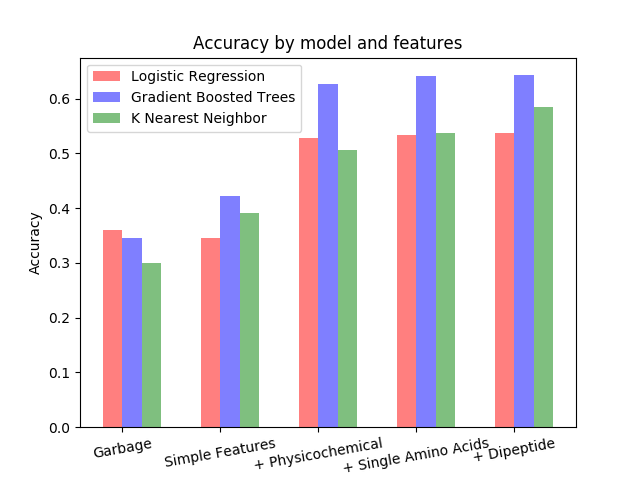
\includegraphics[width=9cm]{histogram}
  \caption{Accuracy of different models and feature sets. Increasing number of features as the histograms move right.}
\end{figure}

\section{Results}

The accuracies reported in Table 1. are the average test accuracies from the ten runs.
The gradient boosted algorithm performed very well under the full feature set, acheiving an accuracy of 0.642724.
This was only marginally better than when it trained on the features without dipeptide statistics.

Looking at the models, gradient boosted trees were consistently more accurate.
The logistic regression model trailed with most feature sets.
This is likely due to the assumption it makes about linear relationships between features.
Some features, like a high or low dipeptide count, are more categorical, which breaks the linear assumption.
Nearest neighbor did well, but could not match gradient boosted trees.
With more fine tuning of the parameters I wouldn't be surprised if nearest neighbor scored essentially the same as gradient boosted trees.

At the end of the day, gradient boosted trees have won out.
They are a favourite of the Kaggle data competition crowd for the effect we see here.
They eke out slightly more accurate models than competitors with the same features.

Looking to the confusion plot in Figure 2., we can explore some of the most confused classes.
Mitochondrial and nuclear proteins in particular are confused with cytoplasmic proteins.
Secreted and nuclear proteins were the most accurately identified locations.

In Figure 1. we see the effects of adding new feature sets on each model.
The accuracy increases for each set, with some regressions, but with diminishing returns.

\begin{figure}[H]
  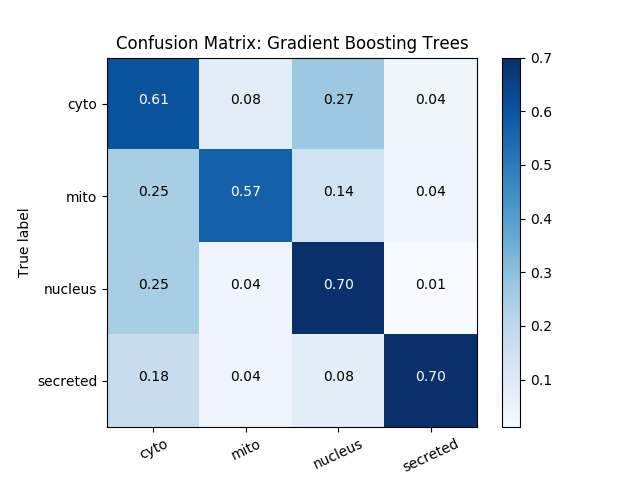
\includegraphics[width=9cm]{confusion}
  \caption{Confusion matrix for different classes predicted by Gradient Boosted Trees with the full feature set.}
\end{figure}

\section{Discussion}

It is not surprising that larger feature sets created more accurate predictions.
What was surprising is that the ordering of how we add feature sets creates a similar effect.
Adding single amino acid, dipeptide, or physicochemical features alone creates a huge jump in accuracy.

A garbage set of features were included to find the lower limit of the models.
It was important to understand how a poor model would perform to ensure my model was doing well.
I was pretty proud of my first model obtaining 40\% accuracy, until I realized guessing "nucleus" every time would get about 35\%.

Whatever our choice for the first feature set, the remaining features provide diminishing returns.
This means there is an overlap in the information provided by data sets.
Whatever signal exists in the raw sequences can be partially extracted from any one of the three data sets, causing this effect.

The diminishing returns of each additional feature sets suggests an alternative approach is necessary to generate substantial improvements.
We might turn to models that are better at interpreting longer sequence information, such as markov models or recurrent neural networks.

We might try to add explicit secondary and tertiary structure features.
Secondary structures like alpha helices and beta sheets are local structures.
Predicting their existence relies heavily on an amino acids immediate neighbors.
This type of information could be picked up by shallow trees with the features in this report, but it is unlikely.
Tertiary structure features result from widely spread dependencies in a sequence.
Predicting their existence could depend on the presence of a feature anywhere in the entire sequence, and were almost definitely not picked up in these models.

Signal peptides, mentioned above, might improve our prediction ability.
The shallow trees I've used in this model will not be able to identify short sequences like signal peptides.
We can incorporate them manually, or ensure the structure of non-parametric models can recognize their presence, like in a Convolutional Neural Network.

\section{Conclusion}

Overall, for relatively simple analysis and simple models, the predictive abilities of this approach were very high.
Each of the feature sets were singularily important, but the benefit they provide was not fully independent, there's overlap.
In the case of gradient boosted trees, dipeptide information was almost useless after having included other amino acid and physicochemical features.

And, finally, the blind predictions are:
\begin{lstlisting}
  SEQ677 Cyto Confidence 55% 
  SEQ231 Secr Confidence 67% 
  SEQ871 Mito Confidence 41% 
  SEQ388 Nucl Confidence 50% 
  SEQ122 Cyto Confidence 37% 
  SEQ758 Nucl Confidence 56% 
  SEQ333 Cyto Confidence 39% 
  SEQ937 Cyto Confidence 77% 
  SEQ351 Cyto Confidence 64% 
  SEQ202 Cyto Confidence 34% 
  SEQ608 Mito Confidence 51% 
  SEQ402 Nucl Confidence 48% 
  SEQ433 Secr Confidence 61% 
  SEQ821 Secr Confidence 55% 
  SEQ322 Nucl Confidence 83% 
  SEQ982 Nucl Confidence 95% 
  SEQ951 Cyto Confidence 52% 
  SEQ173 Cyto Confidence 73% 
  SEQ862 Mito Confidence 66% 
  SEQ224 Cyto Confidence 57% 
\end{lstlisting}

\bibliography{Bioinformatics}

\section{Appendix}

The code for this project can be found at \url{https://github.com/andreweskeclarke/bioinformatics_assignment}.

\end{document}
